\documentclass[lang=en]{sjtuarticle}
\title{A Survey of Distributed PKI}
\author{Log Creative}
\sjtusetup{info/date={2024-05-19}}
\graphicspath{{figs/}}
\usepackage[style=ieee]{biblatex}
\addbibresource{ref.bib}
\usepackage[colorlinks]{hyperref}
\begin{document}
\maketitle

\tableofcontents*

\section{Main challenges}

Public Key Infrastructure (PKI) is ``a set of policies, processes, software, and workstations
used for the purpose of administering certificates and public-private key pairs, including the ability to
issue, maintain, and revoke public key certificates\cite{nist}.''

\subsection{Traditional PKI (PKIX)}

The deployment of PKI on the Internet has been dominated by the ITU-T X.509 standard \cite{pkix}, known as PKIX. A traditional PKIX is composed of five main components: Certificate Authority (CA), Server, Registration Authority (RA), Client, and Repository. However, PKI is not a silver bullet for security and there are several challenges \cite{ellison2000ten}.

\paragraph{CAs are the corruptible central points of failure.} This is the major challenge of traditional PKIs. There have been CA failures across those years \cite{pkixsurvey}, like key leakage, email spoofings, null prefix attacks, internal system compromise, cryptographic flaws, etc. Once the CA is down, then the authentication will not be performed. Virtually all Internet software now relies on these centralized authorities.

\paragraph{Cyber-attacks.} The traditional PKIX architecture may suffer from various cyber attacks \cite{pkixsurvey}: CA Compromises; Compelled Certificate Attack; BGP Route Hijacking; Dangling DNS Record Attack, Deprovisioned cloud instance attack, Expired domain attack, Discontinued service attack; DNS Record Spoofing Attack; Split-World Attack; DNS Cache Poisoning Attack; Vantage Point Downgrade Attack; Truststore Attack; Malicious CA Insertion Attack; Revocation Information Blocking Attack; Zombie Certificate Attack;Efail Attack.

\paragraph{Centralized PKI lacks scalability and flexibility.} Earlier
traditional public key infrastructure was a challenge to be deployed \cite{Gupta2023}.  The centralized system is very vulnerable facing various attacks in the context of scalability and flexibility. Some companies spend significant resources fighting security breaches caused
by misbehaving CAs mentioned earlier \cite{dpki}.

\paragraph{CA Authority is an issue.} There are questions about the authority of CAs to grant specific
authorizations in the certificates they issue. And the CA itself may not be trustworthy as well.

\paragraph{PKI users may not ensure the private key.} The PKI user in all likelihood
do not claim a safe figuring framework with physical access controls, protecting,
air divider, organize security, and different insurances; client stores the private key
on an ordinary PC which is of great possibility a hot environment compared to a physically isolated code environment. Therefore there is a risk that the private key may be leaked by accident.


\subsection{DPKI}

Distributed Public Key Infrastructure (or Decentralized Public Key Infrastructure, DPKI) makes use of use blockchains and other forms of distributed consensus to provide the same functionality
of centralized systems like X.509 while also providing improved scalability and removing \textbf{singe points of failure} for a more secure system \cite{dpkisota}. With the advent of DPKI, \textbf{scalability and flexibility} issues have been addressed.
However, some old implementations of DPKI could still have flaws and face several challenges \cite{dumitrescu2024failures}:

\paragraph{SPKI} Simple Public Key Infrastructure (SPKI) \cite{Ellison1999} to bind privileges or rights (access control) to the public key.  However,
this approach is \textbf{never finalized} and later merged with the simple distributed
security infrastructure (SDSI) \cite{sdsi} that deals with groups and group-membership
certificates. SDSI is the first step towards
a decentralized public key infrastructure, allowing entities
to make local decisions about access control based on their
local policies and knowledge, rather than relying on a central
authority for all decisions. However, there could still be \textbf{a problem of trust} (country in this case).

\paragraph{Log-based PKI.} The log-based PKI provides
transparency and accountability by creating publicly available logs for the generated
certificates. This approach greatly suffers from \textbf{deployment challenges} and
\textbf{certificate revocation issues}. The PKISN (PKI Safety Net) \cite{Szalachowski2016} also follows the same footsteps as in log-based PKI, but proposes an approach to solve the certificate revocation problem when a
trusted CA's private key is compromised. However, this approach as well suffers from the same
\textbf{deployment issues}.

\section{SOTA of DPKI}

The current state-of-the-art (SOTA) of DPKI are smart contract DPKI, QChain, and DKS-PKI.

\subsection{Smart Contract DPKI}

\paragraph{Description.}

The first provably secure DPKI based on smart contracts \cite{patsonakis2018towards} was proposed in 2017, but it is RSA-based and impractical to implement for large-scale projects. A Merkle-tree based smart contract DPKI \cite{Patsonakis2019} was proposed later to reduce the computational cost. This allows for the size of the smart contract state, which is the most expensive resource to access on the
blockchain, to be minimized as well as make sure its security.

The core idea is \textbf{decoupling the storage} of (identity,public-key)
pairs \textbf{from the verification} of their validity. The storage of information relevant to the protocol, e.g.,
(identity,public-keys) pairs, is offloaded to an external database
component, which is modeled as unreliable database (\textit{UDB}). Based on Hash-tree accumulator, clients can perform, locally, additions and deletions of elements and supply the smart contract
with appropriate witnesses which prove that the operations
were performed honestly. To generate all involved witnesses,
clients query \textit{UDB} for the history of operations. The accumulator's underlying data structure (Merkle tree) is a balanced,
binary tree, with the accumulator's value represented as the hash of the root node and witnesses are
hash paths starting from a node leading up to the root node. This leads to constant size accumulator
values, but witnesses have $\mathcal{O}(\lambda\log(n))$ bit size where $n$ is the number of accumulated elements and $\lambda$ is the security parameter. Figure \ref{fig:smart} shows the \textsf{Constructor}, \textsf{Register}, \textsf{Revoke}, and \textsf{RetrieveState} operations.

\begin{figure}[h]
    \centering
    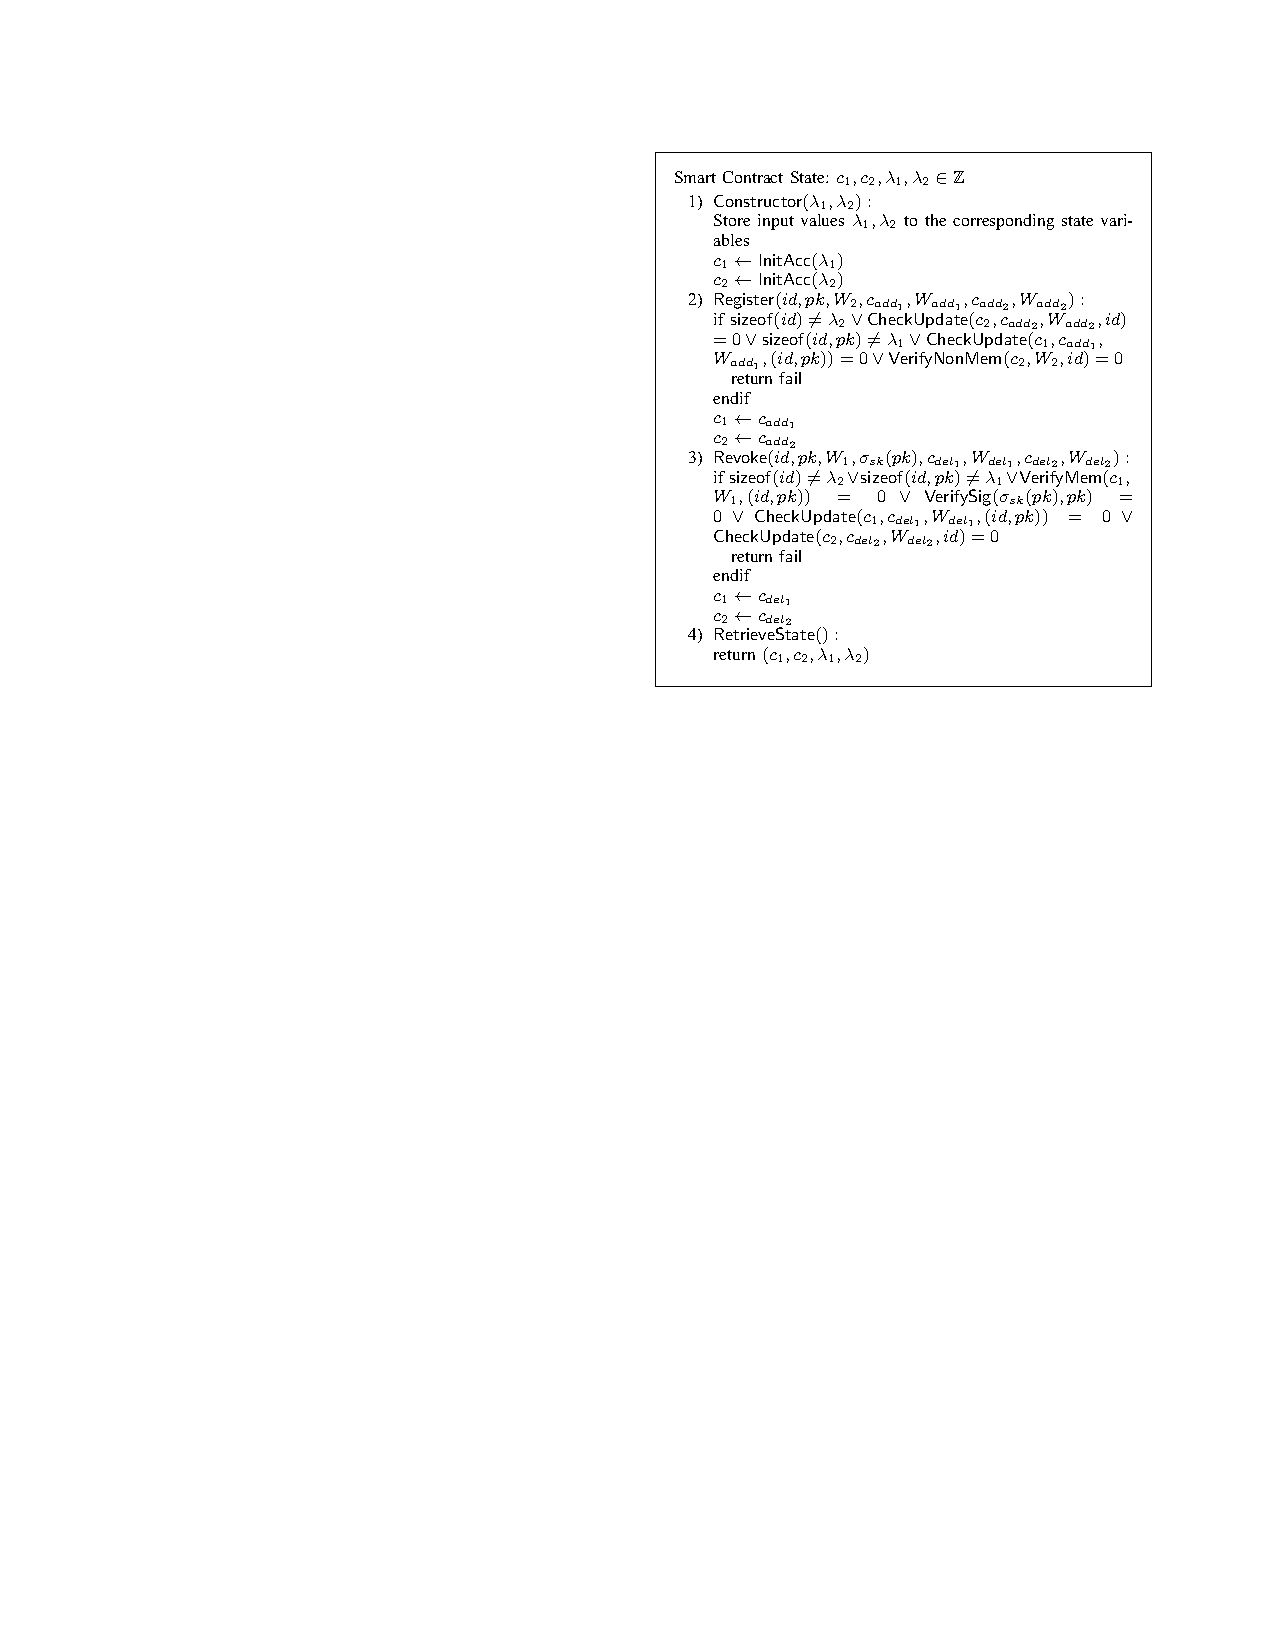
\includegraphics{smart.pdf}
    \caption{Pseudocode of the smart contract DPKI in the hash-based construction}
    \label{fig:smart}
\end{figure}

\paragraph{Advantage.}

It is found that this implementation could easily and securely be used on
Ethereum's mainchain, particularly if developers of the project were willing to make changes that would allow for a DPKI to be faster and more efficient.

\paragraph{Disadvantage.}

However, one challenge that remains is
witnesses being dependent on the number of id-key pairs registered ($\mathcal{O}(\lambda\log(n))$ mentioned earlier), which can become verbose over
time unless steps are taken to ``reset'' the accumulators from time-to-time.

\subsection{QChain}

\paragraph{Description.}

QChain (Quantum-resistant Blockchain-based DPKI) \cite{an2018qchain} is its own blockchain system where each block stores the id-pk pairs and uses their hashes for the Merkle
hash tree structure, while it is secure against quantum computing attacks by modified GLP signature with NTT (Number Theoretic Transformation) \cite{ntt} operations. 

% GLP signature is believed to be secure against side-channel attacks till now. To increase its performance, the modified GLP signature with NTT (Number Theoretic Transformation)  operations is used.

Figure \ref{fig:QChain} illustrates a typical use case of QChain to setup secure communication. The first operator initiates the genesis
block as well as setting up the parameters for the overall
chain. Then, QChain creates another block and users run \textsf{QChain.User.Setup()} and \textsf{QChain.User.Add()}
algorithms in order to register a public key. These keys can be verified using \textsf{QChain.User.Verify()} which
allows users to determine if a key they are provided is authenticated or not.

\begin{figure}[h]
    \centering
    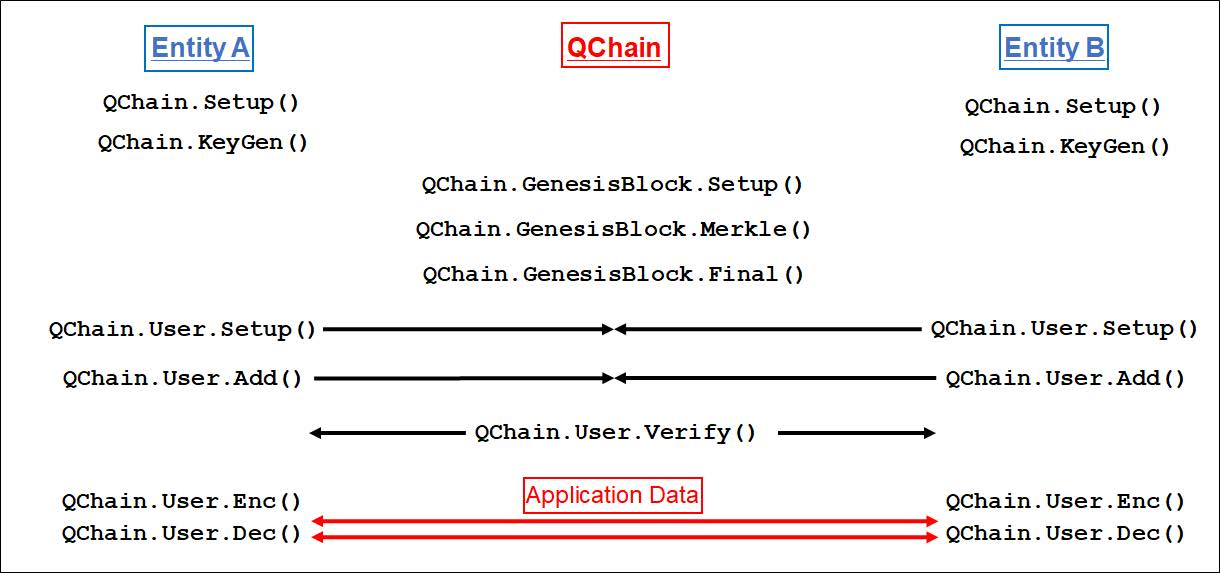
\includegraphics{QChain.jpg}
    \caption{A typical use case of QChain to setup secure communication.}
    \label{fig:QChain}
\end{figure}

\paragraph{Advantage.} It can keep \textbf{offline states} (except for the initiation
of the genesis block) while X.509 v3 must keep online states (particularly by a trusted third party like CA)
in order for users to verify public keys. The construction uses extended X.509 certificate, which makes it \textbf{easy to integrate} with current X.509 standards. It does \textbf{prevent single points of failure}, which is an inherent
problem with X.509.

On the other hand, it is \textbf{quantum-resistant} by using NTT operations.

\paragraph{Disadvantage.} There is no security proof for the protocol provided by the authors and therefore there is a possibility for non-quantum based adversaries to trick the system into accepting malicious
registrations or for an adversary to deceive users by using a non-current association of a public key \cite{dpkisota}. It does not seem clear how the immutable property of QChain allows for users to revoke associations. 

\subsection{DKS-PKI}

\paragraph{Description.}

DKS-PKI (Distributed Key Server for PKI) \cite{Faisal2022} utilizes a consensus-based distributed network of authority nodes, permissioned
storage nodes, and publicly accessible key-server nodes to ensure
that the certificate registration/issuance, storage, distribution, and revocation
mechanisms are secure, transparent, and fault-tolerant. All the certificates
(registered public keys) in DKS-PKI are accessible using their associated
unique identifiers (UIDs) through the key-server nodes.

% The architecture shown in Figure \ref{fig:dks-pki} consists of four types of nodes: authority nodes (ANs); transaction repository nodes (TxRNs); broadcasting nodes (BNs); and key-server nodes (KSNs). 

In the architecture shown in Figure \ref{fig:dks-pki}, the authority nodes (ANs), the transaction repository
nodes (TxRNs), and the key-server nodes (KSNs) communicate to each
other through the broadcasting nodes (BNs) only. However, the same type of
nodes may have direct communication channels (e.g., AN-AN, TxRN-TxRN,
BN-BN) between them for data synchronization.

\begin{figure}[h]
    \centering
    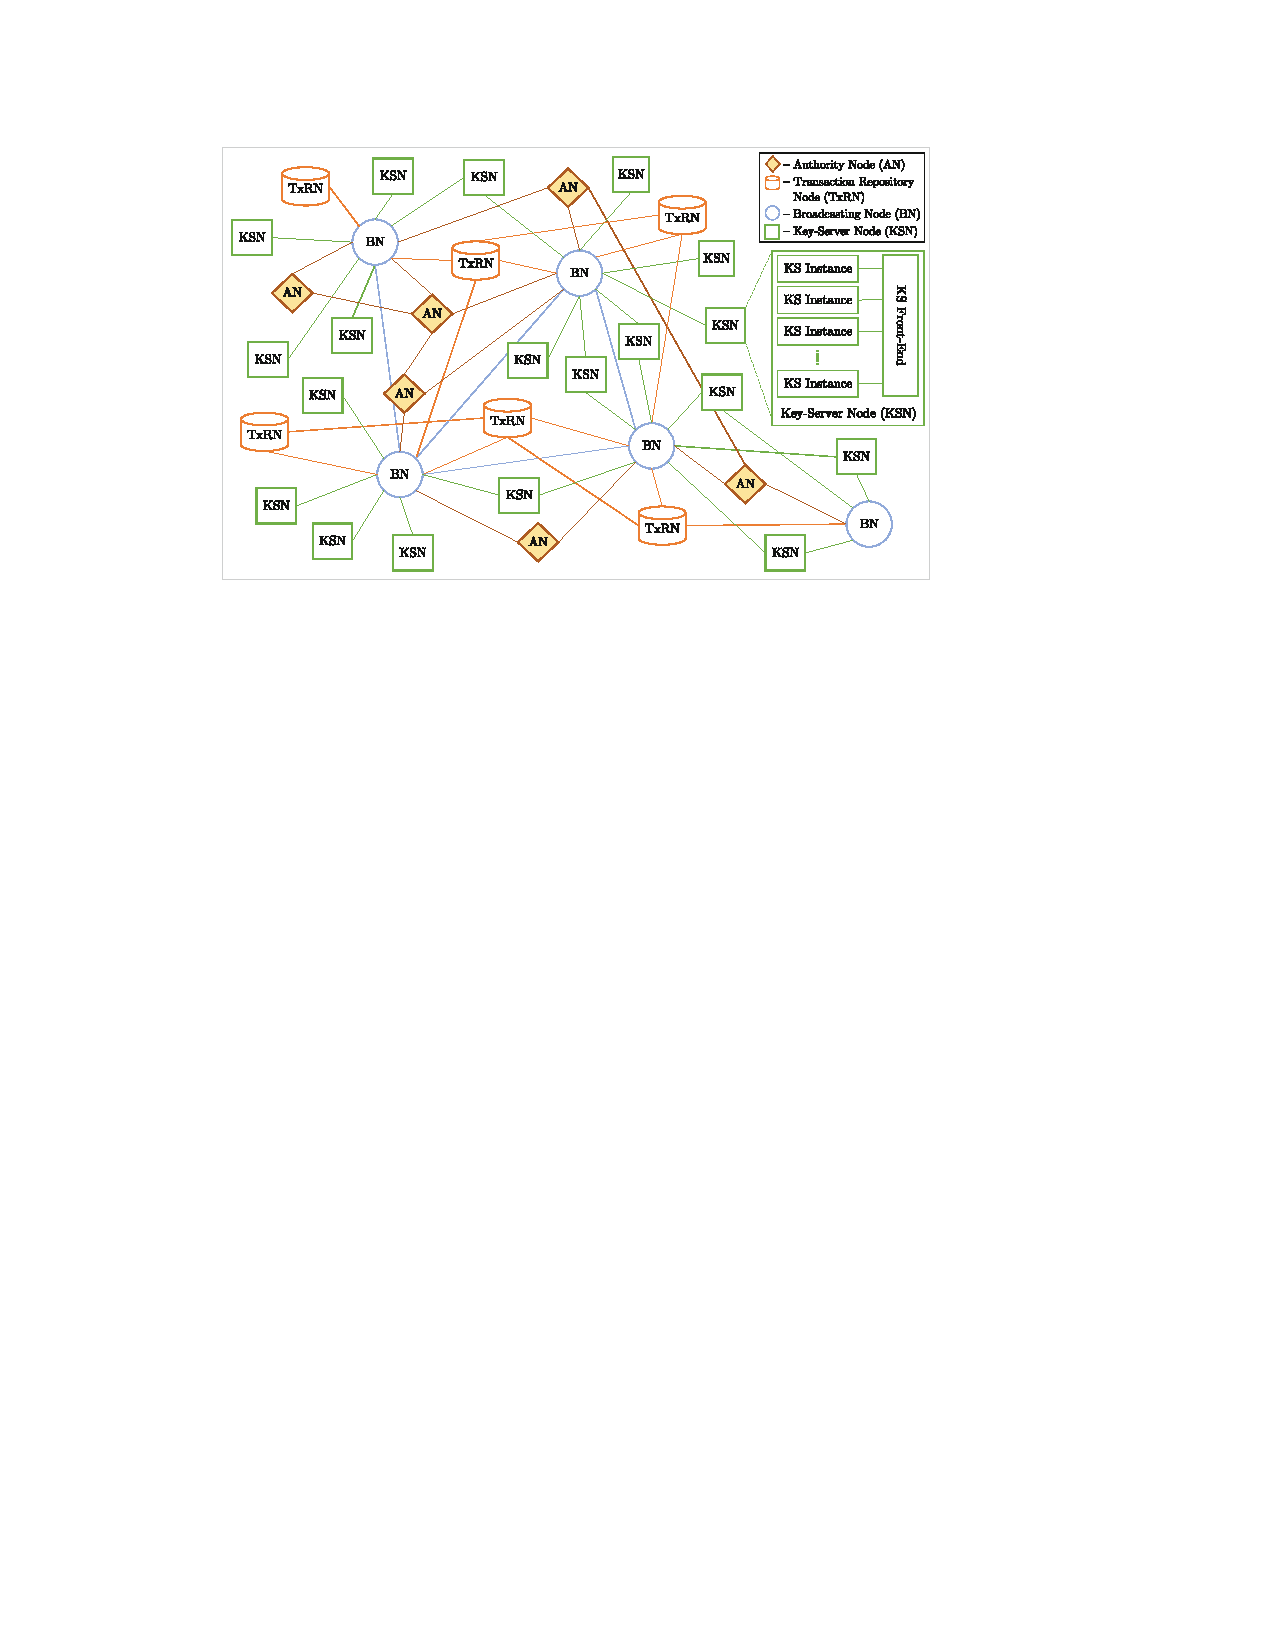
\includegraphics{DKS-PKI.pdf}
    \caption{Architecture of DKS-PKI}
    \label{fig:dks-pki}
\end{figure}

When the BNs receive an incoming message
from a subscribed node, they publish this message to the other subscribed
nodes only. Each AN validates certificate registration and revocation requests
submitted to it. For each registration request, it generates a public key certificate
and its associated 256-bit unique identifier (UID). Then, the AN generates
a temporary transaction enclosing these information.

After validating registration/revocation
requests, the ANs broadcast temporary transactions enclosing entity information
and their signed public key certificates to the other ANs and the TxRNs.
After successful consensus between the ANs, the TxRNs generate the sealed
transactions from these temporary transactions.

Then, the TxRNs store these sensitive entity information, issued or revoked
certificates, and their associated UIDs permanently. The TxRNs also transmit
the issued certificates and their associated UIDs to the KSNs. These KSNs need to be
publicly available at all times and are responsible to manage certificate requests
from anywhere in the world.

\paragraph{Advantage.} There are two major challenges for CA-based PKIs: (a) increased intermediate CAs gives
rise to the possibility that the mis-issuance of certificates or the disclosure of
any such trusted CAs' private keys can cause serious problems to the security
of internet communications; (b) these CAs have ample powers to maliciously or erroneously issue
duplicate certificates or revoke the existing certificates without the owner's consent.

This architecture solves the two major problems with the existing CA-based
PKI:
(a) This proposed architecture ensures
transparency and accountability of the certificate issuers (authority nodes). Any
authority node (AN) cannot issue certificates in the network without reaching
consensus with the other ANs. This approach \textbf{solves the certificate mis-issuance
problem}. (b) Next, certificate revocation is effective as soon as the authority nodes
reach a consensus on the revocation transaction. After that, the revoked certificates
are separated from the rest of the issued certificates in the TxRNs and the
KSNs. This \textbf{solves the certificate revocation issue} as well.

The \textbf{performance} of the certificate distribution mechanism
shows reasonable results with the increasing number of certificate requests. 

The distributed architecture
\textbf{prevents DoS/DDoS attacks} on any node and improves the availability of the
PKI network for authentication.

% and eliminates the need for having any hierarchical intermediate CAs
% that can issue any certificates to anyone. It ensures accountability of the certificate
% issuers and allows the system to detect any mis-issuance of certificates
% as well as any revocation of certificates promptly.

\paragraph{Disadvantage.} It is relatively different from the PKIX architecture, which may introduce the difficulty of making it widely adopted.

\printbibliography

\end{document}